\documentclass[10pt,twocolumn,twoside]{genpaper}
\usepackage[sort&compress]{natbib}

\usepackage{flushend}
\usepackage{xcolor,colortbl}
\usepackage{subfig}
\usepackage{longtable}
% For pseudocode
\usepackage[linesnumbered,boxed,ruled,vlined]{algorithm2e}
\newcommand\mycommfont[1]{\footnotesize\ttfamily\textcolor{blue}{#1}}
\SetCommentSty{mycommfont}
% For code embedding (Bash, Java...)
\usepackage{listings}
\lstset{basicstyle=\ttfamily,
  showstringspaces=false,
  commentstyle=\color{red},
  keywordstyle=\color{blue}
}
\usepackage{mathtools}


\definecolor{Gray}{gray}{0.9}
\newcommand{\npscarf}{$\mathtt{npScarf}$}
\newcommand{\npscarfg}{$\mathtt{npScarf\_wag}$}
\newcommand{\npreader}{$\mathtt{npReader}$}
\newcommand{\npanalysis}{$\mathtt{npAnalysis}$}
\newcommand{\npbarcode}{$\mathtt{npBarcode}$}
\newcommand{\npgraph}{$\mathtt{npGraph}$}
\newcommand{\canu}{$\mathtt{Canu}$}
\newcommand{\unicycler}{$\mathtt{Unicycler}$}
\newcommand{\spades}{$\mathtt{SPAdes}$}
\newcommand{\albacore}{$\mathtt{Albacore}$}
\newcommand{\racon}{$\mathtt{Racon}$}
\newcommand{\metrichor}{$\mathtt{Metrichor}$}
\newcommand{\minimap}{$\mathtt{minimap2}$}
\newcommand{\miniasm}{$\mathtt{miniasm}$}
\newcommand{\bwa}{$\mathtt{BWA\text{-}MEM}$}

\newcommand{\ec}{\emph{E.~coli}}
\newcommand{\sce}{\emph{S.~cerevisae}}
\newcommand{\kp}{\emph{K.~pneumoniae}} 

\newcommand{\IE}{\emph{i.e.}}
\newcommand{\EG}{\emph{e.g.}}
\newcommand{\review}[1]{\textcolor{red}{#1}}

\title{Online resolving assembly graph by long reads data}
\shorttitle{Real-time Scaffolding with Assembly graph}

%Authors
\author[1]{Son Hoang Nguyen}
\author[1]{Minh Duc Cao}
\author[1,$\ast$]{Lachlan Coin}

%Affiliation
\affil[1]{Institute for Molecular Bioscience, the University of Queensland, 
St Lucia, Brisbane, QLD 4072 Australia}

\correspondingauthor{
\textsuperscript{$\ast$}
To whom correspondence should be addressed. 
E-mails: author.last@email.com,author.first@email.com
}

%To show compiled date
\compiledate

\begin{document}
%Abstract and keywords have to be defined before \maketitle

\onecolumn
\renewcommand{\figurename}{Supplementary Figure}
\renewcommand{\tablename}{Supplementary Table}
%\setcounter{page}{1}
%\setcounter{figure}{0}
%\setcounter{table}{0}
% 
\begin{center}
 \Large{Supplementary Notes}
\end{center}
%%%%%%%%%%%%%%%%%%%%%%%%%%%%%%%%%%%%%%%%%%%%%%%%%%%%%%%%%%%%%%%%%%%%%
%%%%%%%%%%%%%%%%%%%%%% text supplementary %%%%%%%%%%%%%%%%%%%%%%%%%%%
\section{Supplementary Note 1: Distance metric for clustering algorithm}\label{supp:note1}
%%Move to Supplementary
Assume there are 2 Poisson distributions $P_1$ and $P_2$ with density functions $$p_1(x,\lambda_1)=\frac{e^{-\lambda_1}\lambda_1^x}{\Gamma(x+1)}$$ and $$p_2(x,\lambda_2)=\frac{e^{-\lambda_2}\lambda_2^x}{\Gamma(x+1)}$$ 
The Kullback-Leibner divergence from $P_2$ to $P_1$ is defined as:
$$D_{KL}(P_1||P_2)=\int_{-\infty}^{\infty} p_1(x)\log{\frac{p_1(x)}{p_2(x)}} dx$$
or in other words,  it is the expectation of the logarithmic difference between the probabilities $P_1$ and $P_2$, where the expectation is taken with regard to $P_1$.

The log ratio of the density functions is
$$\log{\frac{p_1(x)}{p_2(x)}}=x\log{\frac{\lambda_1}{\lambda_2}}+\lambda_2-\lambda_1$$
take expectation of this expression with regard to $P_1$ with mean $\lambda_1$ we have
$$D_{KL}(P_1||P_2)=\lambda_1\log{\frac{\lambda_1}{\lambda_2}}+\lambda_2-\lambda_1$$

The metric we used is the distance defined as
$$D(P_1,P_2)=\frac{D_{KL}(P_1||P_2)+D_{KL}(P_2||P_1)}{2}=\frac{1}{2}(\lambda_1-\lambda_2)(\log{\lambda_1}-\log{\lambda_2})$$

\section{Supplementary Note 2: Coverage re-estimation}\label{supp:note2}
The re-estimation is basically carried out by following two steps.
\begin{itemize}
\item[1.] From nodes coverage, estimate edges' value by quadratic unconstrained optimization of the least-square function:
$$\frac{1}{2}\sum_{i}{l_i((\sum{e^{+}_{i}}-c_i)^2+(\sum{e^{-}_{i}}-c_i)^2}$$
where $l_i$ and $c_i$ is the length and coverage of a node $i$ in the graph;

$\sum{e^{+}_{i}}$ and $\sum{e^{-}_{i}}$ indicates sum of the values of incoming and outgoing edges from $i$ respectively. 
The above function and be rewritten as:
$$f(x)=\frac{1}{2}x^TQx + b^Tx + r$$
and then being minimized by using gradient-based method.
\item[2.] Update nodes' coverage based on itself and its neighbor edges' measures.
\end{itemize}
The calibration is iterative until no further improvements are made or a threshold loop count is reached.

\section{Supplementary Note 3: Contigs binning}\label{supp:note3}
We implemented a simple binning algorithm based on the clustered contigs, the graph topology as well as statistics calculated by length and coverage of each contigs. The algorithm works well for isolate or simple mock metagenomics, but not robust enough for complicated community.

On the other hand, if external binning algorithm is employed, the resulting output must be converted into a text file that specifies the corresponding bin of every contigs, just like output from MetaBAT. By that, each line of the file would be:
$
\mathtt{<contig\_ID>} \; ~ \mathtt{<bin\_ID>}
$
where $\mathtt{bin\_ID}=0$ indicates unspecified binned contigs.

\section{Supplementary Note 4: Constructing bridges in real-time}\label{supp:note4}
We implemented a data structure to represent the connection between two unique contigs in the assembly graph, namely \emph{bridge}. 
A bridge has 4 levels of completion, ranging from 1 to 4 depends on how close to finish it is.
When a new bridge is built with only one anchor (unique ending), it has level 1.
If both anchor nodes are identified, its completion level is 2.
Only then, a path finding algorithm is applied to find candidate paths of this bridge. When potential paths (more than 1) are listed successfully, the completion level is increased to 3.
Finally, when the only path solution is determined out of all candidates, the bridge is assigned as complete-built with level 4.

At early stages (level 1 or 2), a bridge is constructed progressively by alignments from long reads that spanning its corresponding anchor(s).
In an example from Figure~\ref{figure:npgraph_merging}, bridges from a certain anchor (highlighted in red) are created by extracting appropriate alignments from incoming long reads to the contigs. Each of the steps therefore is assigned a weighing score based on its alignment quality.
Due to the error rate of long reads, there should be deviations in terms of steps found and spans measured between these bridges, eventhough they represent the same connection.
A continuous merging phase, as shown in the figure, takes advantage of a pairwise Needleman-Wunsch dynamic programming to generate a consensus list based on weight and position of each of every stepping nodes. The spans are calibrated accordingly by averaging out the distances. On the other hand, the score of the merged steps are accumulated over time as well.
Whenever a consensus bridge is anchored by 2 unique contigs at both ends and hosting a list of steps with sufficient coverage, it is ready for a path finding in the next step.

\begin{figure}[!hpt]
\centering
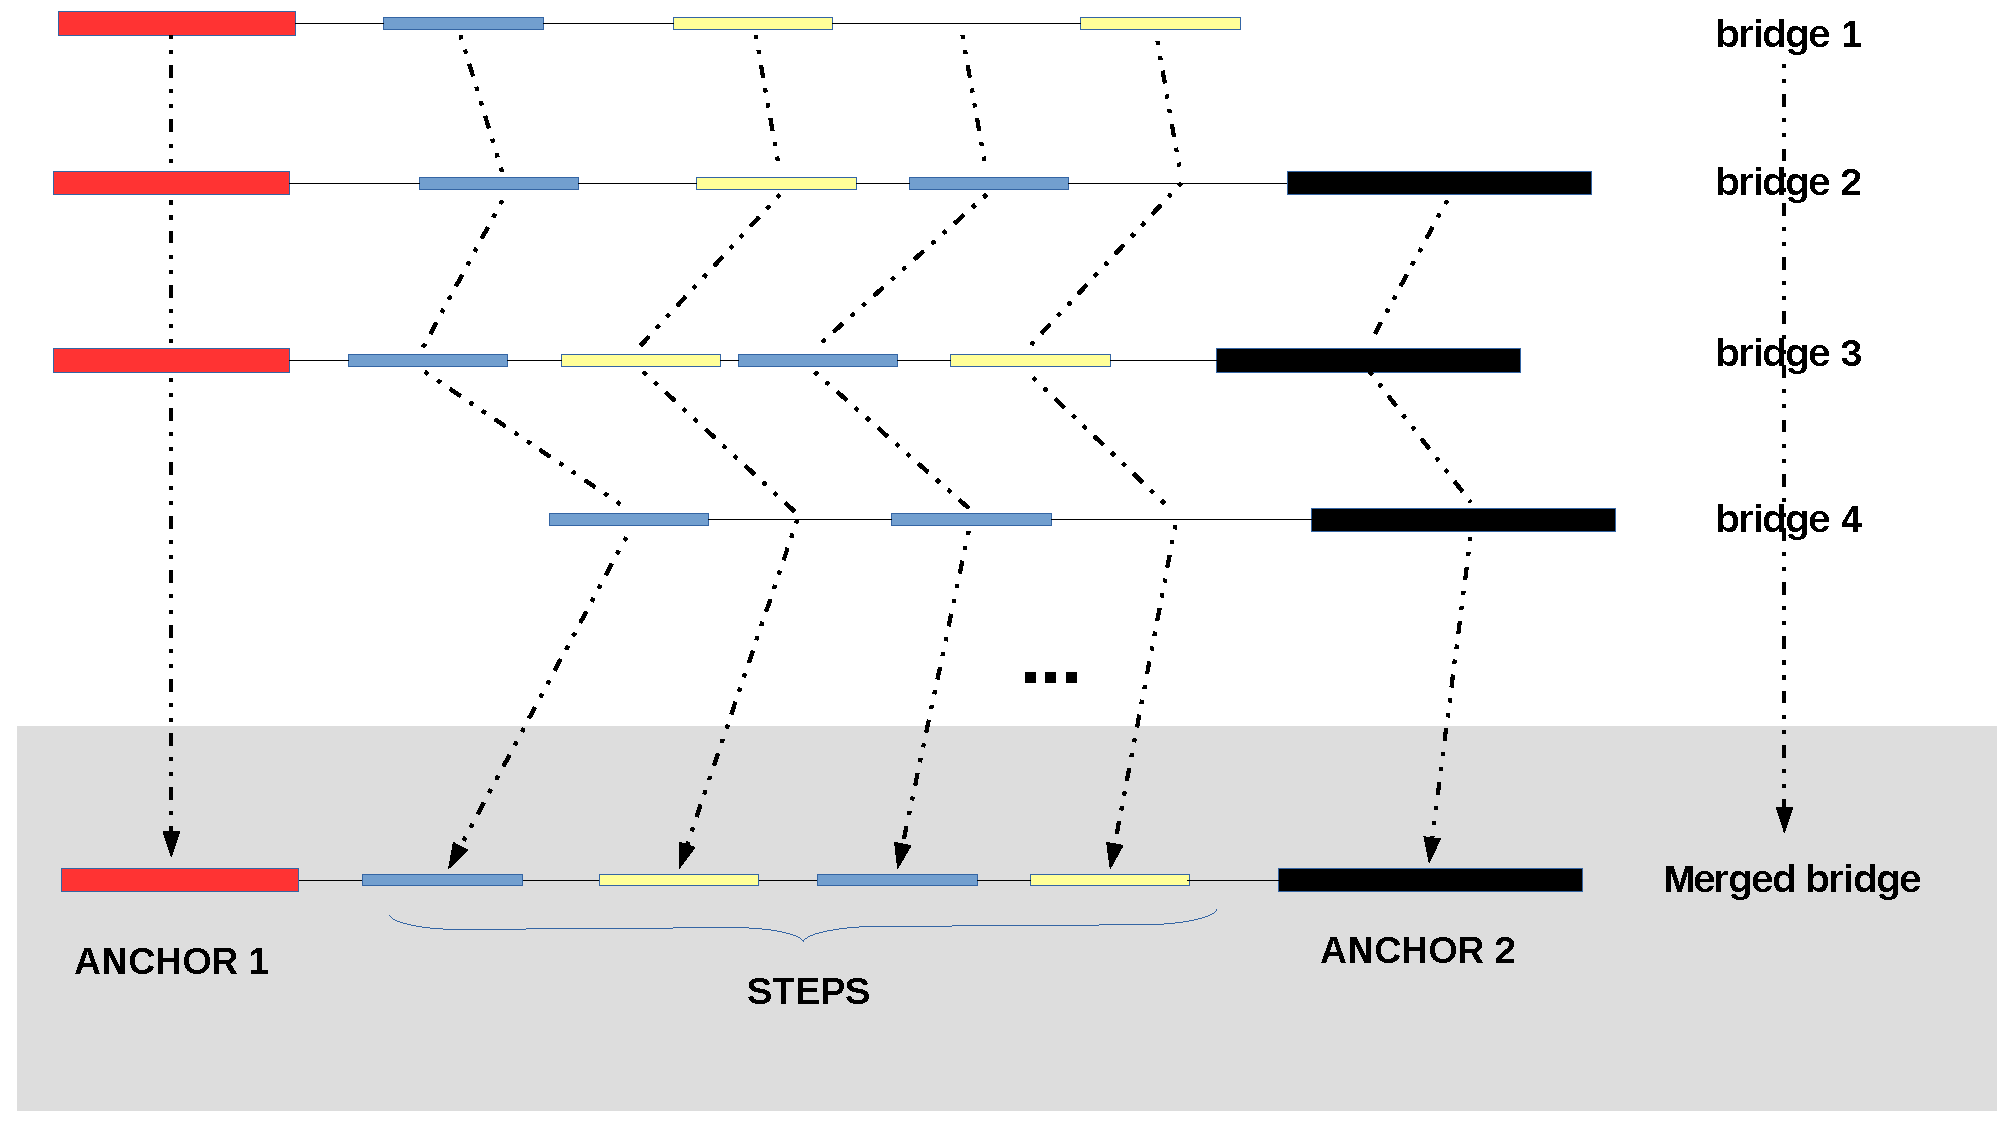
\includegraphics[width=.8\textwidth]{images/bridge_merging.pdf}
\caption[Example of bridge merging progressively]{Bridge merging progressively in real-time. Sequencing long reads induce alignments to the contigs where new bridges are created respectively. Bridges sharing same anchors can be merged together to form the ultimate, more comprehensive bridge (with more spans and better approximation about distances between them).}
\label{figure:npgraph_merging}
\end{figure}


\section{Supplementary Note 5: Path finding algorithm}\label{supp:note5}
However, due to false alignments from shorter contigs to the long reads, not all of the reported step nodes are neccessary to appear in the ultimate path resolved by the bridge. 
In most cases, the accumulated score of each step indicates its likelihood to be the true component of the final solution.
For that reason, a strategy similar to binary searching is employed to find a path across 2 anchors of a bridge.


\begin{algorithm}[!hpt]
\DontPrintSemicolon
\KwData{Assembly graph $G\{V,E\}$}
\KwIn{Pair of bidirected nodes $\overrightarrow{v_1}, \overrightarrow{v_2}$ and estimated distance $d$ between them}
\KwOut{Set of candidate paths connecting $\overrightarrow{v_1}$ to $\overrightarrow{v_2}$ with reasonable distances compared to $d$}
\SetKwFunction{DFS}{DFS} 
\SetKwProg{Fn}{Function}{:}{}
\Fn{\DFS{$\overrightarrow{v_1}, \overrightarrow{v_2}$, $d$}}{
$P$:=new List()\;
$M$:=$\mathtt{shortestTree}(\overrightarrow{v_2},d)$ \tcp*{build shortest tree from $\overrightarrow{v_2}$ with range $d$}
\If{$M.contain(\overrightarrow{v_1})$}{
    $S$:=new $Stack()$ \tcp*{stack of sets of edges to traverse}
    $edgesSet$:=$getEdges(\overrightarrow{v_1})$ \tcp*{get all bidirected edges going from $\overrightarrow{v_1}$}
    $S.push(edgesSet)$\;
    $p$:=new $Path(\overrightarrow{v_1})$ \tcp*{init a path that has $\overrightarrow{v_1}$ as root}
    \While{true}{
        $edgesSet$:=$S.peek()$\;
        \If{$edgesSet.isEmpty()$}{
            \If{$p.size() \leq 1$}{
                $\mathbf{break}$ \tcp*{stop the loop when there is no more edge to discover}
            }
        $S.pop()$\;
        $d$+=$p.peekNode.length()+p.popEdge().length()$\; 
        }
        \Else{
            $curEdge \coloneqq edgesSet.remove()$\;
            $\overrightarrow{v}$:=$curEdge.getOpposite(p.peekNode())$\;
            $S.push(getEdges(\overrightarrow{v}).includedIn(M))$\;
            $p.add(curEdge)$\;
            \If{reach $\overrightarrow{v_2}$ with reasonable $d$}{
                $P.add(p)$\;
            }
            $d$-=$\overrightarrow{v}.length()+curEdge.length()$\;
        }
    }
}

\Return{$P$}
}
\caption{Pseudo-code for finding paths connecting 2 nodes given their estimated distance.}
\label{algo:findpath}
\end{algorithm}

Algorithm~\ref{algo:findpath} generally demonstrates the path finding algorithm for two nodes given their estimated distance. In which, function 

$\mathtt{shortestTree}(\overrightarrow{vertex},distance) : (V,Z) \rightarrow V^n$ 

from line 3 of the algorithm's pseudo code builds a shortest tree rooted from $\overrightarrow{v}$, following its direction until a distance of approximately $d$ (with a tolerance regarding nanopore read error rate) is reached. This task is implemented based on Dijkstra algorithm.
This tree is used on line 4 and in function $includedIn()$ on line 19 to filter out any node or edge with ending nodes that do not belong to the tree.

Basically, the algorithm keeps track of a stack that contains sets of candidate edges to discover. During the traversal, a variable $d$ is updated as an estimation for the distance to the target. A hit is reported if the target node is reached with a reasonable distance \IE{} close to zero, within a given tolerance (line 21). 
A threshold for the traversing depth is set (150) to ignore too complicated and time-consuming path searching.

Note that the $length()$ functions for node and edge are totally different. While the former returns the length of the sequence represented by the node, \IE{} contig from short-read assembly, the latter is usually negative because an edge models a link between two nodes, which is normally an overlap (except for composite edges). For example, in a \emph{k-mers} SPAdes assembly graph, the value of an edge is $-k+1$. 

\section{Supplementary Note 6: Graph decomposing for output report}\label{supp:note6}
A path $p=\{v_0,e_1,v_1,\ldots,v_{k-1},e_k,v_k\}$ of size $k$ is considered as straight if every edge along the path, $e_i, \forall i=1,\ldots,k$, must be the only option to traverse from either $v_{i-1}$ or $v_i$ following the transition rule.
To decompose the graph, we can just simply mask out all incoming/outgoing edges rooted from any node with in/out degree greater than 1 as demonstrated in Figure~\ref{figure:npgraph_decompose}. These edges are defined as branching edges which stop straight paths from further extending.

\begin{figure}[!hpt]
\centering
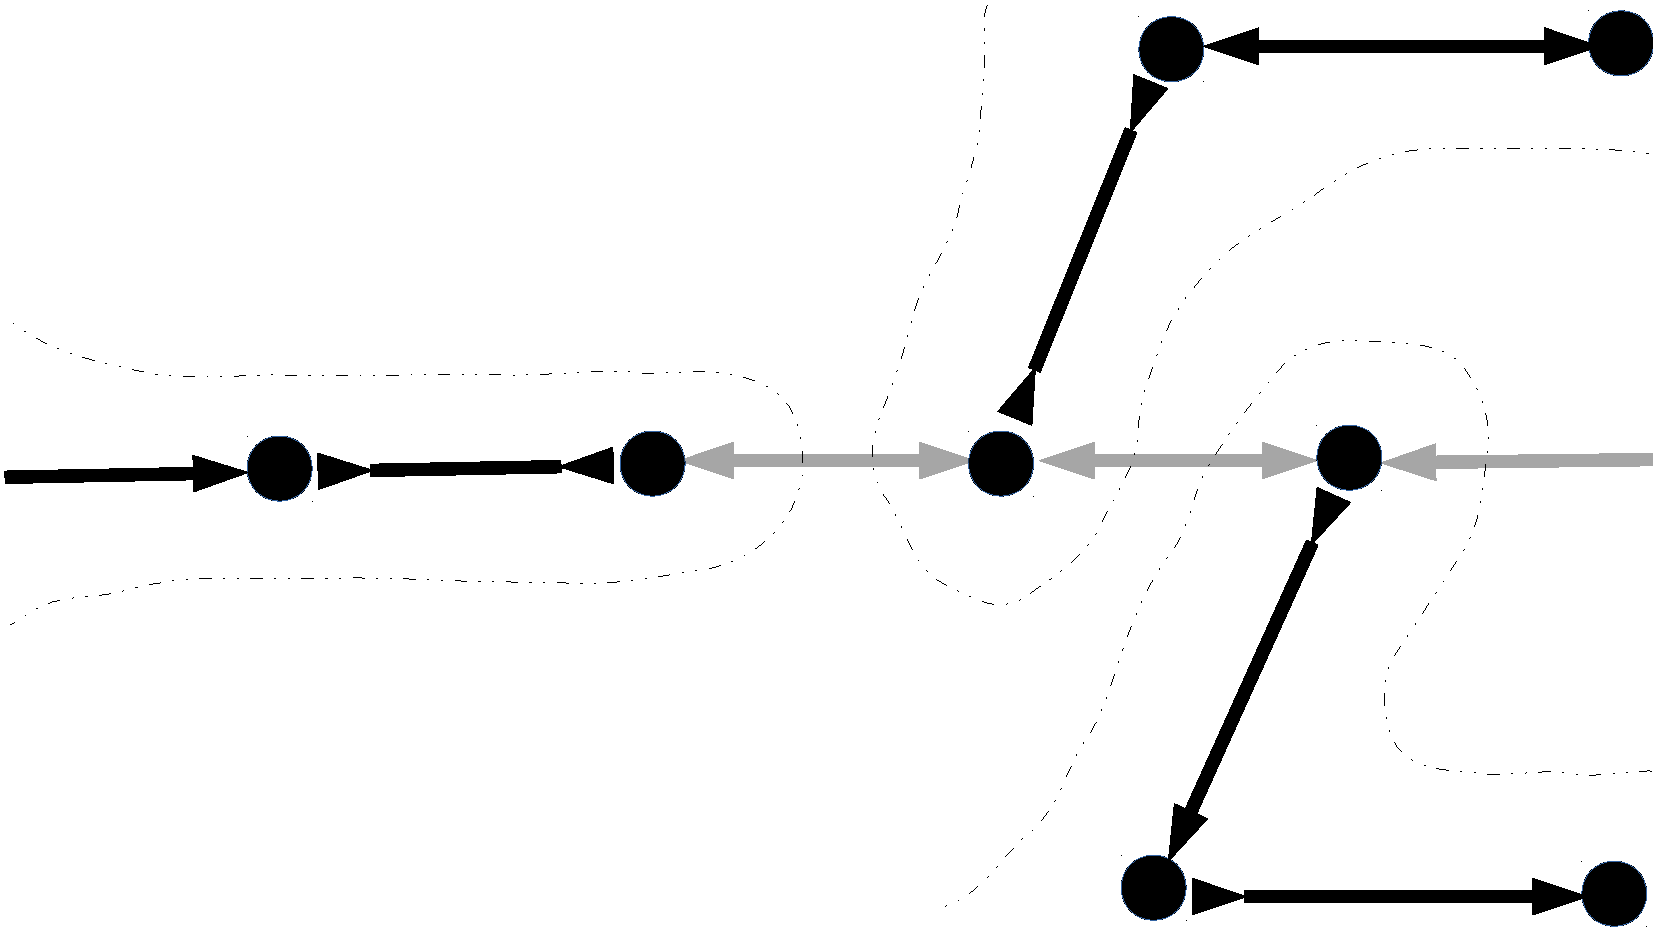
\includegraphics[width=.6\textwidth]{images/decompose.pdf}
\caption[Example of graph decomposition into longest straight paths]{Example of graph decomposition into longest straight paths. Branching edges are masked out (shaded) leaving only straight paths (bold colored) to report. There would be 3 contigs extracted by traversing along the straight paths here.}
\label{figure:npgraph_decompose}
\end{figure}
The decomposed graph is only used to report the contigs that can be extracted from an assembly graph at certain time point. For that reason, the branching edges are only masked but not removed from the original graph as they would be used for further bridging.

%%%%%%%%%%%%%%%%%%%%%%%%%%%%%%%%%%%%%%%%%%%%%%%%%%%%%%%%%%%%%%%%%%%%%
%%%%%%%%%%%%%%%%%%%%% figures & tables %%%%%%%%%%%%%%%%%%%%%%%%%%%%%%
\clearpage
\newpage
\setcounter{figure}{0}
\setcounter{table}{0}
% 
\begin{center}
 \Large{Supplementary Figures and Tables}
\end{center}

\makeatletter

\newlength\oriarrayrulewidth  
\newcount\orilowpenalty
\newcommand\nobreakmidrule{%
 \noalign{\global\oriarrayrulewidth\arrayrulewidth\relax
          \global\orilowpenalty\@lowpenalty\relax  
          \global\@lowpenalty=\numexpr-10000\relax%
          \global\arrayrulewidth\lightrulewidth\relax}
 \hline
 \noalign{\global\@lowpenalty=\orilowpenalty\relax%
          \global\arrayrulewidth\oriarrayrulewidth\relax}}

\makeatother


\begin{longtable}[!hpt]{llcrrrrr}
\caption{Benchmarking \npgraph{} against \npscarf{} versions, $\mathtt{hybridSPAdes}$ and \unicycler{} hybrid assembler with the synthetic data set.}
\label{supp_tab:synthetic_benchmark}\\
\toprule
    &       & Assembly &  & N50  & Mis- &  Mismatch & Indel \\
    & Method & size (bp) & \#Contigs  & (bp) & assemblies & (per $100$Kbp) & (per $100$Kbp) \\
    \hline  
\endfirsthead
\multicolumn{8}{c}%
{\tablename\ \thetable\ -- \textit{Continued from previous page}} \\
\hline
    &       & Assembly &  & N50  & Mis- &  Mismatch & Indel \\
    & Method & size (bp) & \#Contigs  & (bp) & assemblies & (per $100$Kbp) & (per $100$Kbp) \\
\hline
\endhead
\hline \multicolumn{8}{r}{\textit{Continued on next page}} \\
\endfoot
\hline
\endlastfoot

\rowcolor{Gray}
\multicolumn{8}{l}{random sequences no repeats} \\* %
\nobreakmidrule
\rowcolor{Gray}
& npScarf &  4110000 &  3  &  4000000  &  0  & 0.00  & 0.00\\*
\rowcolor{Gray}
& npScarf\_wag & 4109516  &  3  &  4000000  &  0  & 0.00  & 0.00\\*
\rowcolor{Gray}
& npGraph-bwa & 4110000  &  3  &  4000000  &  0  & 0.00  & 0.00\\*
\rowcolor{Gray}
& npGraph-mm2 & 4110000  &  3  &  4000000  &  0  & 0.00  & 0.00\\*
\rowcolor{Gray}
& hybridSPAdes & 4110231  &  3  & 4000077   &  0  & 0.00  &  0.07\\*
\rowcolor{Gray}
& Unicycler & 4110000  &  3  &  4000000  &  0  & 0.00  &  0.00\\
\hline
\multicolumn{8}{l}{random sequences some repeats} \\* %
\nobreakmidrule
& npScarf & 4110940  &  3  &  4002715  &  0  &  0.00 &  0.66\\*
& npScarf\_wag & 4437094  &  7 &  2795129  &  0  &  0.00 &  1.07\\*
& npGraph-bwa & 4110000  &  3  &  4000000  &  0 &  0.00 &  0.00\\*
& npGraph-mm2 &  4110000 &  3  &   4000000 & 0  & 0.00  &  0.00\\*
& hybridSPAdes & 4107566  &  3  &  3999364  &  0  & 0.02  & 0.02\\*
& Unicycler &  4110000 &  3 & 4000000  &  0 & 0.00  &  0.00\\
\hline
\rowcolor{Gray}
\multicolumn{8}{l}{random sequences many repeats} \\* %
\nobreakmidrule
\rowcolor{Gray}
& npScarf &  4316934 &  8  &  3963485  &  24  & 11.55  & 34.54\\*
\rowcolor{Gray}
& npScarf\_wag &  5215965 &  16  &  1515563  &  37  & 0.32  & 7.22\\*
\rowcolor{Gray}
& npGraph-bwa & 4110000  &  3  &  4000000  &  0  &  0.32 & 0.15\\*
\rowcolor{Gray}
& npGraph-mm2 &  4110000 &  3  &  4000000  &  0  & 0.32  & 0.15\\*
\rowcolor{Gray}
& hybridSPAdes & 4108190  &  3  &  3999621  &  0  &  0.68 &  0.15\\*
\rowcolor{Gray}
& Unicycler & 4110000  &  3  &  4000000  &  0  &  0.32  & 0.15  \\
\hline
% \pagebreak
% \toprule
\multicolumn{8}{l}{\emph{Acinetobacter} A1} \\* %
\nobreakmidrule
& npScarf & 3912299  &  3  &  3870269  &  4  & 4.74  & 13.02 \\*
& npScarf\_wag & 3945166  &  3  &  3906368  &  1  & 7.00  & 14.02 \\*
& npGraph-bwa & 3918374  &  2  &  3909643  &  0 & 16.34  & 0.61 \\*
& npGraph-mm2 & 3885898  &  2  &  3877167  & 1 & 18.05  & 1.03 \\*
& hybridSPAdes &  3929948 &  53  &  3353679  &  0  & 35.48  & 3.22\\*
& Unicycler & 3917745  &  2 & 3909014  & 0  & 2.50  &  0.13\\
\hline
\rowcolor{Gray}
\multicolumn{8}{l}{\emph{Acinetobacter} AB30} \\* %
\nobreakmidrule
\rowcolor{Gray}
& npScarf & 4512464  &  7  &  4304628  &  35  & 57.95  & 72.87\\*
\rowcolor{Gray}
& npScarf\_wag & 5315235  &  13  &  1267710  &  136  &  73.55 & 8.15\\*
\rowcolor{Gray}
& npGraph-bwa & 4335342  &  2  &  4148952  &  1  & 16.93  & 1.45\\*
\rowcolor{Gray}
& npGraph-mm2 & 4335790  &  1  &  4335790  & 0   &  6.97 & 0.25\\*
\rowcolor{Gray}
& hybridSPAdes & 4337369  &  3  &  2701005  &  0  &  12.80 &  1.39\\*
\rowcolor{Gray}
& Unicycler &  4333041 &  1  &  4333041  &  1  &  6.42 &  0.53\\
\hline
\multicolumn{8}{l}{\ec{} K12 MG1655} \\* %
\nobreakmidrule
& npScarf & 4649902  &  2  &  4641702  &  4  & 14.94  & 34.35 \\*
& npScarf\_wag &  4687952 &  3  &  4641732  &  0  & 6.55  &  1.96\\*
& npGraph-bwa & 4641743  &  1  &  4641743  & 0  &  4.50 & 0.43 \\*
& npGraph-mm2 & 4641820  &  1  &  4641820  &  0 &  3.88 & 0.26 \\*
& hybridSPAdes &  4644555 &  1  &  4641036  &  0  & 0.62  & 0.09\\*
& Unicycler & 4641650  &  1 &  4641650 &  0 & 3.43  & 0.26 \\
\hline
\rowcolor{Gray}
\multicolumn{8}{l}{\ec{} O25b H4-ST131} \\* %
\nobreakmidrule
\rowcolor{Gray}
& npScarf &  5245913 &  3  &  5095571  &  7  &  7.05 & 18.81\\*
\rowcolor{Gray}
& npScarf\_wag & 5292700  &  3  &  3469617  &  9  &  9.03 & 1.55\\*
\rowcolor{Gray}
& npGraph-bwa & 5237821  &  7  &  4049493  &  1  &  3.38 & 0.31\\*
\rowcolor{Gray}
& npGraph-mm2 &  5249799 &  3  &  5110117  &  0  &  2.40 & 0.15\\*
\rowcolor{Gray}
& hybridSPAdes & 5252762  &  8  &  4258948  &  2  &  5.43 &  0.57\\*
\rowcolor{Gray}
& Unicycler & 5249442  &  3  &  5109760  &  0  & 4.02 & 0.27 \\
\hline
% \pagebreak
% \toprule
\multicolumn{8}{l}{\emph{Klebsiella} 30660 NJST258 1} \\* %
\nobreakmidrule
& npScarf & 5559772  &  7  &  5259053  &  4  & 17.18  & 13.48\\*
& npScarf\_wag & 5613780  &  7  &  5268535  &  6  & 1.59  & 1.92\\*
& npGraph-bwa & 5534843  &  8  &  5263229  &  0  & 3.15  & 0.76\\*
& npGraph-mm2 & 5534878  &  8  &  5263264  &  0  & 2.75  & 0.74\\*
& hybridSPAdes &  5545668 & 8   &  5545668  &  2  & 4.95  & 0.09 \\*
& Unicycler & 5537860  &  9  &  5263196  &  0  & 1.34  & 0.51 \\
\hline
\rowcolor{Gray}
\multicolumn{8}{l}{\emph{Klebsiella} MGH 78578} \\* %
\nobreakmidrule
\rowcolor{Gray}
& npScarf &  5729304 &  5  &  5316429  &  12  & 14.90  & 20.27\\*
\rowcolor{Gray}
& npScarf\_wag & 5754443  &  5  &  3026286  &  16  &  8.17 & 2.56\\*
\rowcolor{Gray}
& npGraph-bwa &  5695801 &  7  &  5311745  &  1  & 12.65  & 1.25\\*
\rowcolor{Gray}
& npGraph-mm2 & 5696302  &  6  &  5315267  &  0  &  6.06 & 0.44\\*
\rowcolor{Gray}
& hybridSPAdes &  5706470 &  11  &  5315273  &  1  & 3.82  &  0.67\\*
\rowcolor{Gray}
& Unicycler &  5694231 &  14  &  5315096  &  0  & 5.38 &  0.21\\
\hline
\multicolumn{8}{l}{\emph{Klebsiella} NTUH-K2044} \\* %
\nobreakmidrule
& npScarf & 5471696  &  2  &  5249198  &  6  & 4.82  &  8.55\\*
& npScarf\_wag & 5530559  &  3  &  5249369  &  2  &  2.25 &  1.35\\*
& npGraph-bwa & 5472629  &  2  &  5248476  & 0  & 2.52  &  0.31\\*
& npGraph-mm2 &  5472655 &  2  &  5248503  &  0 &  1.21 &  0.26\\*
& hybridSPAdes & 5473572  &  2  &  5248894  &  0  &  0.44 & 0.15\\*
& Unicycler & 5472697  & 2  & 5248545  &  0 & 2.41  &  0.35\\
\hline
\rowcolor{Gray}
\multicolumn{8}{l}{\emph{Mycobacterium tuberculosis} H37Rv} \\* %
\nobreakmidrule
\rowcolor{Gray}
& npScarf &  4498245 &  4  & 4402238   &  8  & 5.15  & 2.68\\*
\rowcolor{Gray}
& npScarf\_wag &  4506056 &  4  &  4410942  &  3  & 6.81  & 2.59\\*
\rowcolor{Gray}
& npGraph-bwa & 4411406  &  1  &  4411406  &  0  & 1.88  & 0.43\\*
\rowcolor{Gray}
& npGraph-mm2 & 4411532  & 1   &  4411532  &  0  & 0.68  & 0.00\\*
\rowcolor{Gray}
& hybridSPAdes & 4413942  &  1  &  4410519  &  0  &  0.75 &  0.11\\*
\rowcolor{Gray}
& Unicycler & 4411538  &  1  &  4411538  &  0  &  2.22 &  0.34\\
\hline
% \pagebreak
% \toprule
\multicolumn{8}{l}{\emph{Saccharomyces cerevisiae} S288c} \\* %
\nobreakmidrule
& npScarf &  11986800 &  24  &  796769  &  51  &  62.12 & 21.46 \\*
& npScarf\_wag & 12003203  &  21  &  917017  &  21  & 69.14  & 5.47 \\*
& npGraph-bwa & 11921736  &  40  &  913090  &  3 &  38.04 &  1.94\\*
& npGraph-mm2 & 11920984  &  38  &  913198  &  2 &  20.66 &  0.95\\*
& hybridSPAdes &  12027533 &  45  &  770543  &  5  & 32.58  & 1.94\\*
& Unicycler &  11847655 & 72  & 909114  &  0 & 21.81  &  1.04\\
\hline
\rowcolor{Gray}
\multicolumn{8}{l}{\emph{Shigella dysenteriae}  Sd197} \\* %
\nobreakmidrule
\rowcolor{Gray}
& npScarf &  4586075 &  173  & 36560   &  55  & 120.14  & 111.59\\*
\rowcolor{Gray}
& npScarf\_wag & 5462918  &  92  &  98791  &  105  &  147.48 & 79.28\\*
\rowcolor{Gray}
& npGraph-bwa & 4564058  &  6  &  4369264  &  5  & 80.64  & 11.16\\*
\rowcolor{Gray}
& npGraph-mm2 & 4558920  &  6  &  4364264  &  7  & 75.51  & 10.98\\*
\rowcolor{Gray}
& hybridSPAdes &  4519131 & 23   &  821249  & 96   & 9.57  &  1.42\\*
\rowcolor{Gray}
& Unicycler & 4560901  & 3   &  4369231  &  0  & 11.88  & 1.05 \\
\hline
\multicolumn{8}{l}{\emph{Shigella sonnei} 53G} \\* %
\nobreakmidrule
& npScarf &  6441461 &  20  &  1953896  &  82  & 164.02  &  219.52\\*
& npScarf\_wag & -  &  -  &  -  &  -  & -  &  -\\*
& npGraph-bwa & 5211544  &   4 &  4988532  & 0  & 14.53  &  0.31\\*
& npGraph-mm2 & 5211527  &  4  &   4988519 & 0  &  8.56 &  0.17\\*
& hybridSPAdes & 5223875  &  8  &  2195455  &  2  & 41.92  & 0.06\\*
& Unicycler &  5220517 &  5 &  4988548 & 0  & 7.39  &  0.52\\
\hline
\rowcolor{Gray}
\multicolumn{8}{l}{\emph{Streptococcus suis} BM407} \\* %
\nobreakmidrule
\rowcolor{Gray}
& npScarf &  2183951 & 3   &  2146594  &  0  & 21.51  & 9.17\\*
\rowcolor{Gray}
& npScarf\_wag & 2289880  &  3  &  1493189  &  1  & 3.17  & 1.96\\*
\rowcolor{Gray}
& npGraph-bwa & 2154623  &  6  &  2131479  &  1  & 5.25  & 0.28\\*
\rowcolor{Gray}
& npGraph-mm2 & 2149876  &  6  &  2146774  &  0  & 1.44  & 0.28\\*
\rowcolor{Gray}
& hybridSPAdes & 2172703  &  2  &  2146237  &  0  & 6.82  &  0.09\\*
\rowcolor{Gray}
& Unicycler &  2170829 &   2 &  2146250  &  0  &  2.67 & 0.32 \\
\hline
\end{longtable}

\begin{figure}[!hpt]
\centering
\subfloat[\emph{Citrobacter~freundii} CAV1374]{
	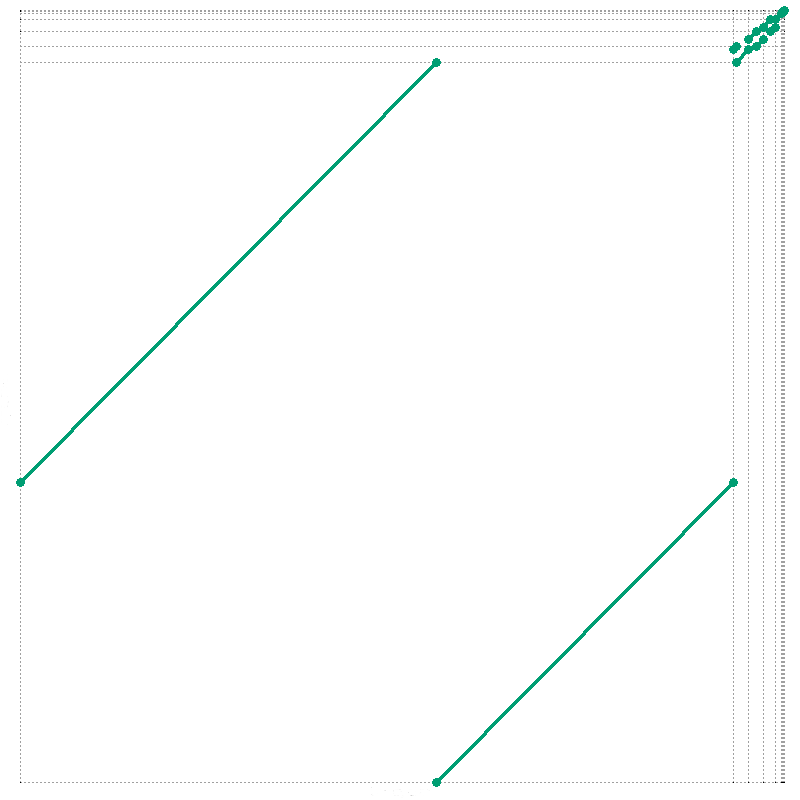
\includegraphics[width=.45\textwidth]{images/dp_c_freundii_cav1374.png}
}
\hfill
\subfloat[\emph{Klebsieall~oxytoca} CAV1015]{
	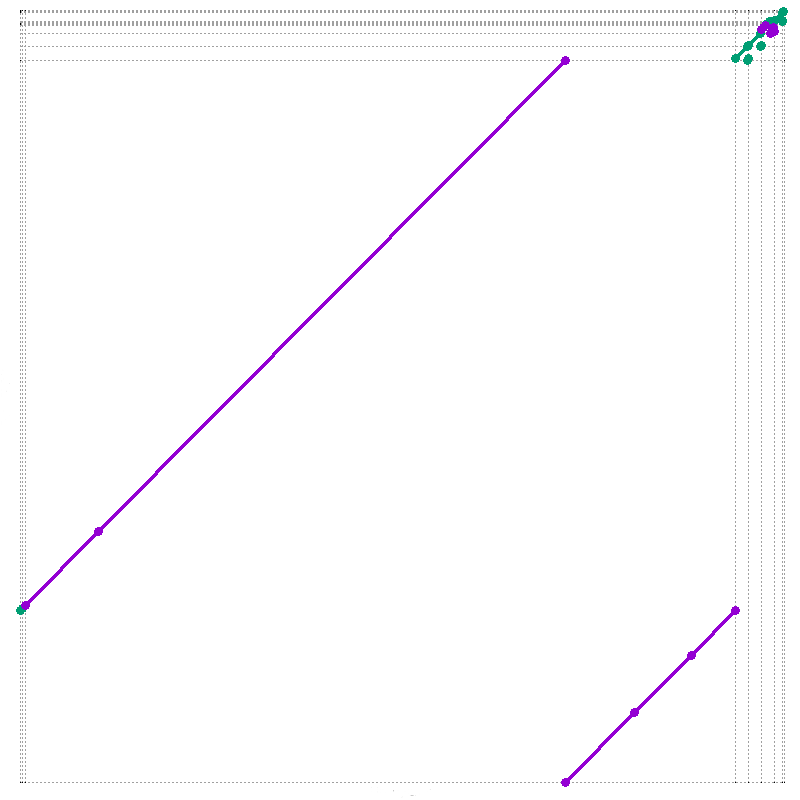
\includegraphics[width=.45\textwidth]{images/dp_k_oxytoca_cav1015.png}
}
\\
\subfloat[\emph{Enterobacter~cloacae} CAV1411]{
	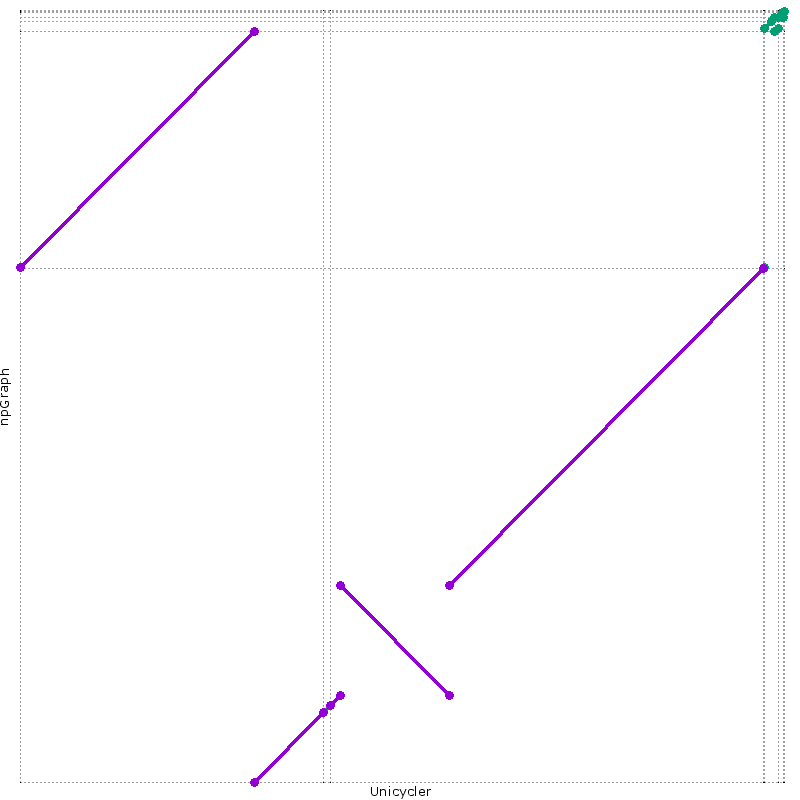
\includegraphics[width=.45\textwidth]{images/dp_e_cloacae_cav1411.png}
}
\caption[Dotplot generated by MUMmer for assembly results of \unicycler{} versus \npgraph{}.]{Dotplot generated by MUMmer for assembly results of \unicycler{} versus \npgraph{}. Structural agreements between two methods were found in (a)~\emph{C.freundii} and (b)~\emph{K.oxytoca} assembly contigs. On the other hand, for (c)~\emph{E.cloacae} sample, there was a disagreement detected between 2 largest contigs given by two assembly algorithms. This case is investigated more thoroughly by using a reference from a same bacterial strain in Figure~\ref{supp_fig:npgraph_ref}.}
\label{supp_fig:npgraph_dotplot}
\end{figure}

\begin{figure}[!hpt]
\centering
\subfloat[\emph{E.~cloacae} \unicycler{} assembly versus reference genome]{
	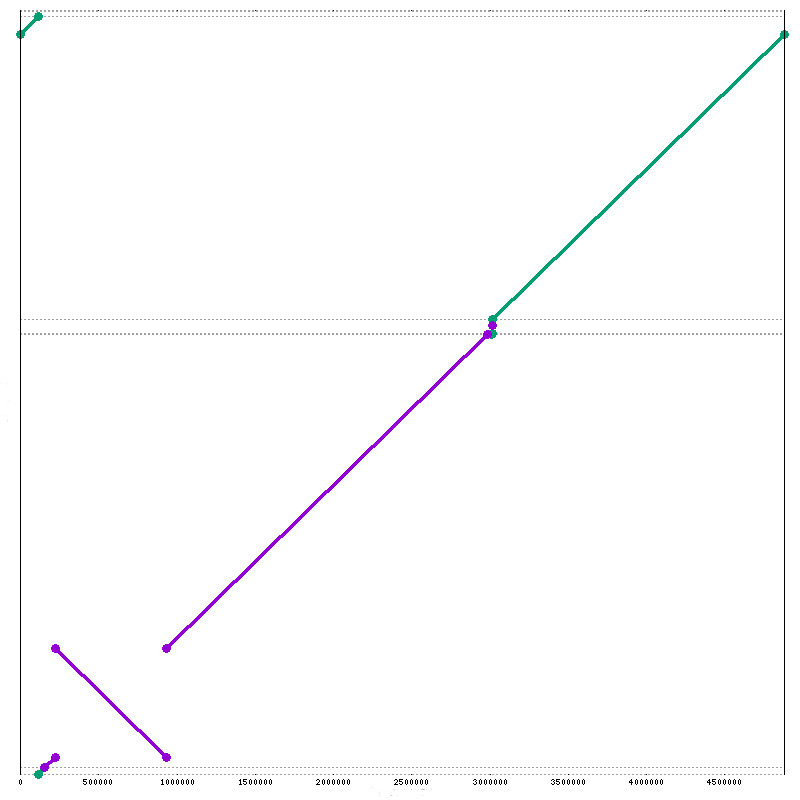
\includegraphics[width=.5\textwidth]{images/dp_ref_unicycler.png}
}
\hfill
\subfloat[\emph{E.~cloacae} \npgraph{} assembly versus reference genome]{
	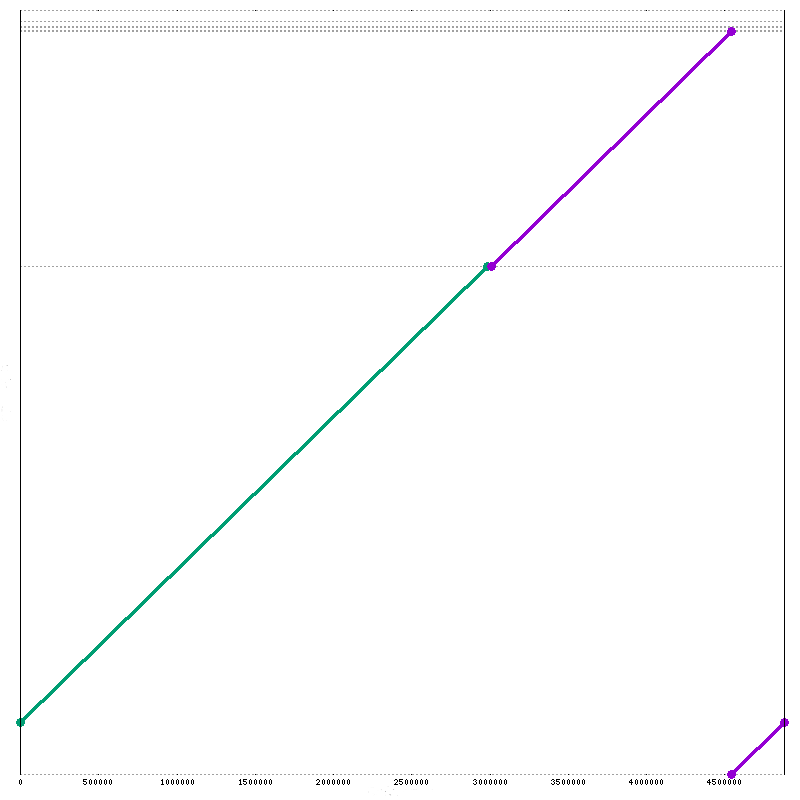
\includegraphics[width=.5\textwidth]{images/dp_ref_npgraph.png}
}
\caption[Alignments of a \emph{Enterobacter~cloacae} reference genome to assembly sequences generated by \unicycler{} and \npgraph{}]{Alignments of an \emph{Enterobacter~cloacae} reference genome to assembly sequences generated by  (a)~\unicycler{} and (b)~\npgraph{}. While the former presents a structural variant, the latter is virtually an 1-to-1 mapping.}
\label{supp_fig:npgraph_ref}
\end{figure}

\end{document}
